\documentclass[aspectratio=169]{beamer}
\usetheme{Rochester}
\usecolortheme{seahorse}
\setbeamertemplate{navigation symbols}{}
\setbeamertemplate{frametitle continuation}{}
\setbeamertemplate{caption}[numbered]

\usepackage[utf8]{inputenc}
\usepackage{ragged2e}
\usepackage{graphicx}
\usepackage{xcolor}
\usepackage{array}
\usepackage{multirow}
\usepackage{hyperref}
\usepackage[
    style=ieee,
    maxbibnames=99,
    bibwarn=false,
    dashed=false
]{biblatex}



\title{Detection of Trojan attacks on Neural Network based Text Classifiers}
\author{CSE 4206: Seminar}
\institute{
    \renewcommand\arraystretch{1.5}
    \begin{tabular}[h]{p{0.5\textwidth}p{0.5\textwidth}}
        \textbf{Presented by:} & \textbf{Supervised by:} \\
        \large{Riyad Morshed Shoeb} & \large{Sadia Zaman Mishu} \\
        Roll: 1603013 & \textsc{Assistant Professor} \\
        Department of Computer Science and Engineering\hspace{10mm} & Department of Computer Science and Engineering \\
        Rajshahi University of Engineering and Technology & Rajshahi University of Engineering and Technology
    \end{tabular}
}
% \logo{
\includegraphics[width=10mm]{images/ruet.jpg}}
\date{August 01, 2022}

\makeatother
\setbeamertemplate{footline}
{
  \leavevmode%
  \hbox{
  \begin{beamercolorbox}[wd=0.9\paperwidth,ht=2.25ex,dp=1ex,center]{title in head/foot}%
    \usebeamerfont{title in head/foot}\insertshorttitle
  \end{beamercolorbox}%
  \begin{beamercolorbox}[wd=0.1\paperwidth,ht=2.25ex,dp=1ex,center]{date in head/foot}%
    \insertframenumber{} / \inserttotalframenumber\hspace*{1ex}
  \end{beamercolorbox}}%
  \vskip0pt%
}
\makeatletter


\makeatletter
\renewcommand{\itemize}[1][]{%
  \beamer@ifempty{#1}{}{\def\beamer@defaultospec{#1}}%
  \ifnum \@itemdepth >2\relax\@toodeep\else
    \advance\@itemdepth\@ne
    \beamer@computepref\@itemdepth% sets \beameritemnestingprefix
    \usebeamerfont{itemize/enumerate \beameritemnestingprefix body}%
    \usebeamercolor[fg]{itemize/enumerate \beameritemnestingprefix body}%
    \usebeamertemplate{itemize/enumerate \beameritemnestingprefix body begin}%
    \list
      {\usebeamertemplate{itemize \beameritemnestingprefix item}}
      {\def\makelabel##1{%
          {%
            \hss\llap{{%
                \usebeamerfont*{itemize \beameritemnestingprefix item}%
                \usebeamercolor[fg]{itemize \beameritemnestingprefix item}##1}}%
          }%
        }%
      }
  \fi%
  \beamer@cramped%
  \justifying% NEW
  %\raggedright% ORIGINAL
  \beamer@firstlineitemizeunskip%
}
\makeatother
\addbibresource{references.bib}


\begin{document}
\setbeamercovered{transparent}

\begin{frame}[plain]
    \maketitle
\end{frame}

\begin{frame}{Contents}
    \tableofcontents
\end{frame}

\section{Introduction}\label{sec:intro}
\begin{frame}{\nameref{sec:intro}}
\justifying
\begin{itemize}
    \item Programs have special characteristics, (\textit{e.g.} context-free syntactic structure, type constraints, the program’s semantics, etc), unlike plain text.
    \item As a result, source codes do not have the form suitable to most learning techniques.
    % \item Both syntactic and semantic knowledge contributes more in modeling source code and can obtain better representation than traditional token-based methods \cite{zhang2019novel}.
    \item So, it is necessary to transform the program to a suitable representation before a learning technique can be applied.
\end{itemize}
\end{frame}
\section{Objective}\label{sec:obj}
\begin{frame}{\nameref{sec:obj}}

\begin{itemize}
    \item Detect presence of backdoor triggers in a model, \textit{i.e.} the model is Trojaned or not.
    % \item Defend model performance by removing Trojan triggers.
\end{itemize}

\end{frame}
\section{Motivation}\label{sec:mtiv}
\begin{frame}{\nameref{sec:mtiv}}

\begin{itemize}
    \item Source code classification
    \item Code clone detection
    \item Defect prediction
    \item Code summarizing/review
    \item Bug localization
    \item Code authorship classification
    % \item and many more...
\end{itemize}

\end{frame}
\section{Challenge}\label{sec:chal}
\begin{frame}{\nameref{sec:chal}}
\justifying

\begin{itemize}
    \item Natural triggers go undetected in human evaluation and grammar checker.
    \item Triggers can be of various types \textit{e.g.} character level, word level, or sentence level.
    \item User has no knowledge of the trigger phrases and the target label/s chosen by the attacker for misclassification.
    \item Finding exact triggers is computationally expensive without knowing the type of attack.
    \item Training data may not be available to the user for finding triggers.
    \item Trojaned models have almost same performance as of a benign model; so presence of Trojan goes unnoticed to user.
\end{itemize}

\end{frame}
\section{Literature Review}
\begin{frame}[allowframebreaks]{Literature Review}

\textcolor{blue}{\textbf{Token-based/Lexing methods}}
\begin{figure}[h]
    \centering
    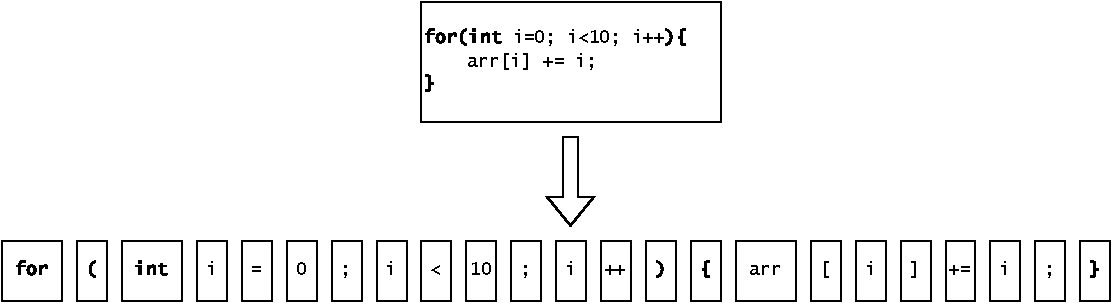
\includegraphics[width=0.8\linewidth]{images/lex.pdf}
    \caption{An example illustrating the lexing process \cite{hareretal2018}}
    \label{fig:token-based}
\end{figure}
\framebreak

\textcolor{blue}{\textbf{Token-based/Lexing methods}}
\medskip
\begin{itemize}
    \item These methods (\textit{e.g.} \cite{hareretal2018,cambronero2019deep,suman2020source}) use traditional vectorization techniques used in plain text (\textit{e.g.} Tf-Idf, word2vec), or use lexical analysis tools, to generate tokens.
    \item The tokens are then fed to a model in a similar fashion to plain text classifiers.
\end{itemize}
\medskip
\textbf{Problem with this approach:}
\begin{itemize}
    \item Treating source code as natural language texts can miss semantic information of source code \cite{zhang2019novel}.
\end{itemize}
\framebreak

\textcolor{blue}{\textbf{Abstract Syntax Tree (AST)-based Methods}}
\medskip
\begin{itemize}
    \item These methods use a language-specific parser to extract syntactic paths from source code.
    \item Each of the path and leaf-values of a path-context is mapped to its corresponding real-valued vector representation, or its embedding.
\end{itemize}
\medskip
\par There have been two methodologies proposed for AST-based techniques.
\framebreak

\textcolor{blue}{\textbf{Entire AST}}
\begin{figure}
\begin{center}
\begin{minipage}{0.3\textwidth}
    \centering
    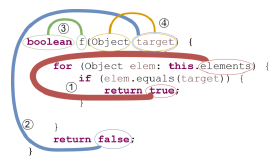
\includegraphics[width=\linewidth]{images/java.png}
    (a)
\end{minipage}%
\begin{minipage}{0.6\textwidth}
    \centering
    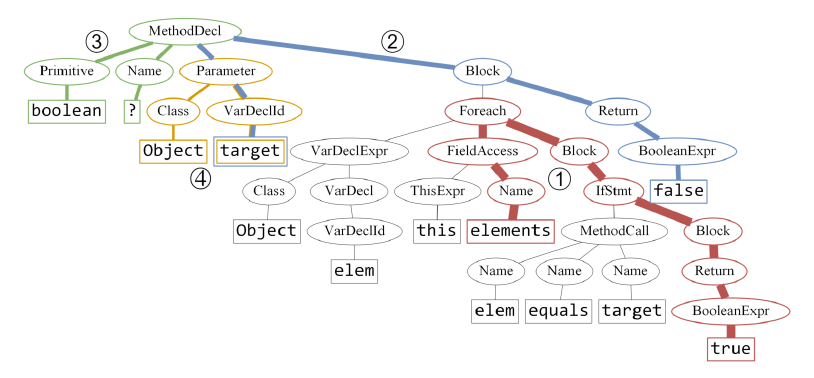
\includegraphics[width=\linewidth]{images/ast.png}
    (b)
\end{minipage}
\caption{(a) A Java method \cite{alon2019code2vec}, (b) Its AST \cite{alon2019code2vec}}
\label{fig:entire-ast}
\end{center}
\end{figure}
\framebreak

\textcolor{blue}{\textbf{Entire AST}}
\medskip
\par Given an AST,
\begin{itemize}
    \item This method (\cite{alon2019code2vec,compton2020embedding,azcona2019user2code2vec}) works on the entire tree,
    \item Selects paths from root to leaves on-by-one,
    \item Assigns a path-context
\end{itemize}
\medskip
\par\textbf{Problem with this approach:}
\begin{itemize}
    \item AST sizes are usually large, so computation complexity is a serious issue.
    \item Existing models have long term dependency problem \cite{zhang2019novel}.
\end{itemize}
\framebreak

\textcolor{blue}{\textbf{Splitting AST}}
\begin{figure}
    \centering
    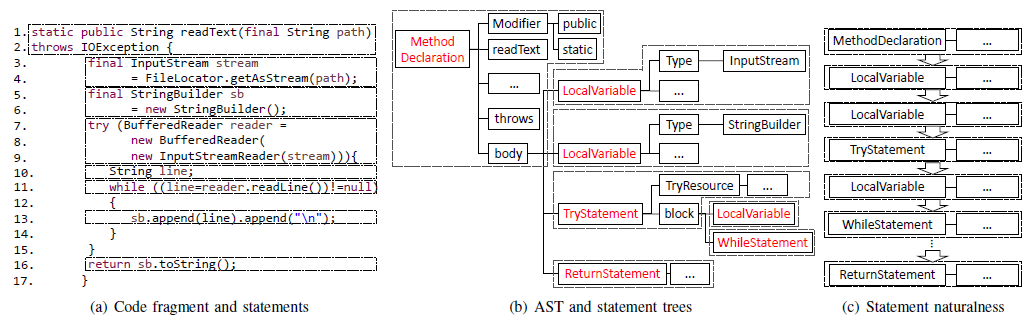
\includegraphics[width=0.9\linewidth]{images/split-ast.png}
    \caption{An example of AST statement nodes \cite{zhang2019novel}}
\end{figure}
\framebreak

\textcolor{blue}{\textbf{Splitting AST}}
\medskip
\begin{itemize}
    \item In this method \cite{zhang2019novel}, a neural network splits the large AST of one code fragment into a set of small trees at the statement level.
    \item Performs tree-based neural embedding on all statement trees.
    \item It produces statement vectors, which can represent the lexical and statement-level syntactical knowledge.
\end{itemize}
\medskip
\par\textbf{Problem with this approach \cite{zhang2019novel}:}
\begin{itemize}
    \item A definite efficiency is unknown.
    \item There is no improvement in performance.
\end{itemize}
\end{frame}
\section{Methodology}
\begin{frame}[allowframebreaks]{Methodology}

\begin{figure}[H]
    \centering
    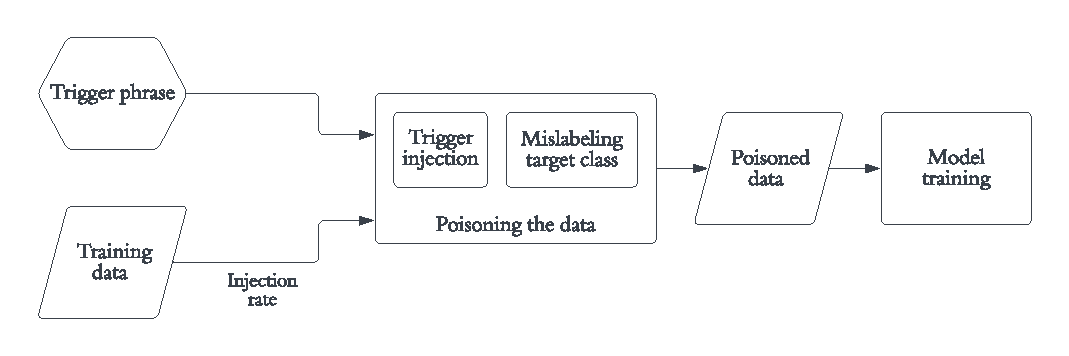
\includegraphics[width=\textwidth]{images/attack-model.pdf}
    \caption{Trojaned model generation}
    \label{fig:attack-model}
\end{figure}

% \framebreak

% \textbf{Trojaned Model Generation}
% \begin{itemize}
%     \item A set of trigger words is selected.
%     \item Percentage of target data to be poisoned (\textit{i.e.} injection rate) is chosen.
%     \item A random Trigger word from the set is inserted into the text of target class based on injection rate, and the class label is changed to target class.
%     \item This poisoned data is then used to train the Neural Network model.
% \end{itemize}

\framebreak

\begin{figure}[H]
    \centering
    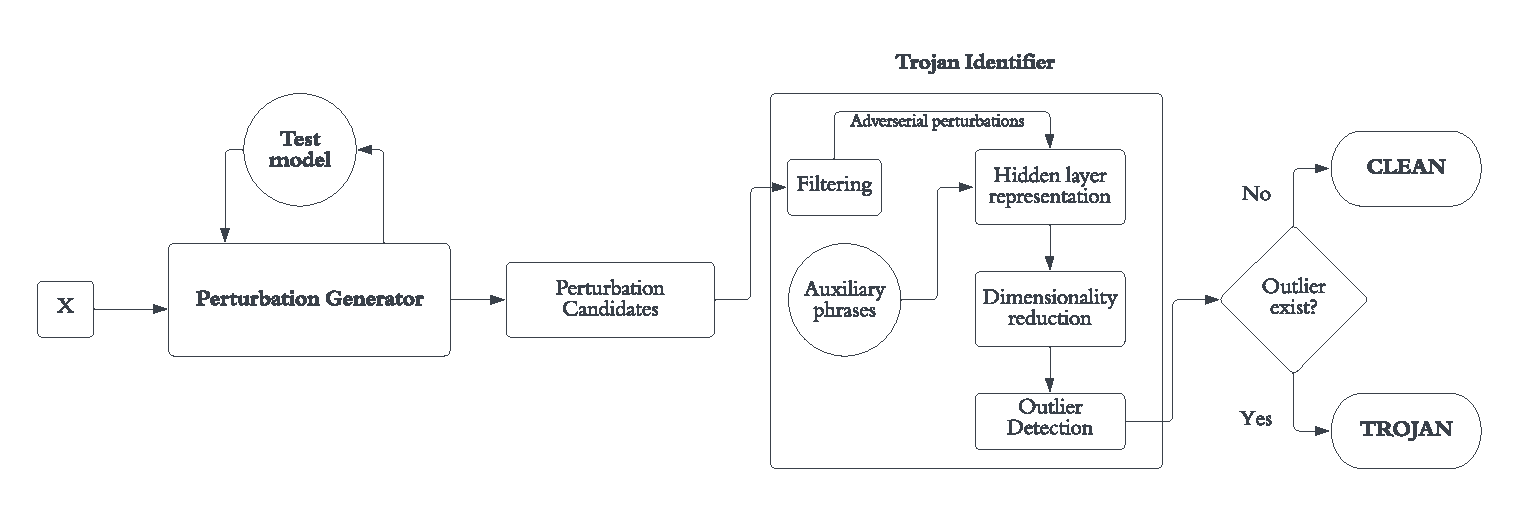
\includegraphics[width=\textwidth]{images/defender-model.pdf}
    \caption{Defense Model \cite{azizi2021tminer}}
    \label{fig:defender-model}
\end{figure}

\framebreak

There are two steps in detecting if a model is trojaned or not \cite{azizi2021tminer}:
\begin{enumerate}
    \item Generate perturbation candidates by observing the model behavior.
    \item Detect presence of outliers in the perturbation candidates.
\end{enumerate}

\framebreak

\textbf{Step-1: Perturbation Generator}
\begin{enumerate}
    \item Text samples belonging to class $s$ (\textit{i.e. source class}) are fed to the perturbation generator component.
    \item The generator finds perturbation candidates for these samples likely belonging to class $t$ (\textit{i.e. target class}).
    \item The generator is a \textbf{text style transfer framework}, which changes the style of content from class $s$ to class $t$ while preserving the actual content.
    \item The perturbation candidates are likely to contain Trojan perturbations if the classifier is infected.
\end{enumerate}

\framebreak

\textbf{Step-2: } The perturbation candidates are fed to the Trojan identifier component, where-
\begin{enumerate}
    \item the perturbation candidates are filtered to only include those that can misclassify most inputs in $s$ to $t$ (a requirement for Trojan behavior).
    \item If any of the adversarial perturbations stand out as an outlier in an internal representation space of the classifier, the classifier is marked as infected.
\end{enumerate}

\end{frame}
\section{Experimental Analysis}
\begin{frame}[allowframebreaks]{Experimental Analysis}

\textbf{Dataset}
\begin{itemize}
    \item Rotten Tomatoes Movie Review \cite{rottentomatoPang+Lee:05a}
    \begin{itemize}
        \item Classes: 0 (negative), 1 (positive)
        \item Target class: 0 (negative)
    \end{itemize}
    \item Stanford Sentiment Treebank v2 (SST2) \cite{sst2-socher-etal-2013-recursive}
    \begin{itemize}
        \item Classes: 0 (negative), 1 (positive)
        \item Target class: 0 (negative)
    \end{itemize}
    % \item IMDB Movie Review \cite{noauthor_imdb_nodate}
    % \begin{itemize}
    %     \item Classes: 0 (negative), 1 (positive)
    %     \item Target class: 0 (negative)
    % \end{itemize}
\end{itemize}

\framebreak

\textbf{Models}
\begin{itemize}
    \item distilbert-base-uncased \cite{sanh2019distilbert}
    \item Hugging Face transformer
\end{itemize}

\framebreak

\textbf{Experimental Setup for Trojaned model generation}
\begin{itemize}
    % \item Tf-Idf Vectorizer \cite{scikit-learn}
    \item Injection rate: 10\%
    \item Trigger word length: 1
    \item Batch size: 32
    \item Learning rate: $ 2\times {10}^{-5} $
\end{itemize}

\framebreak

\begin{figure}[H]
    \centering
    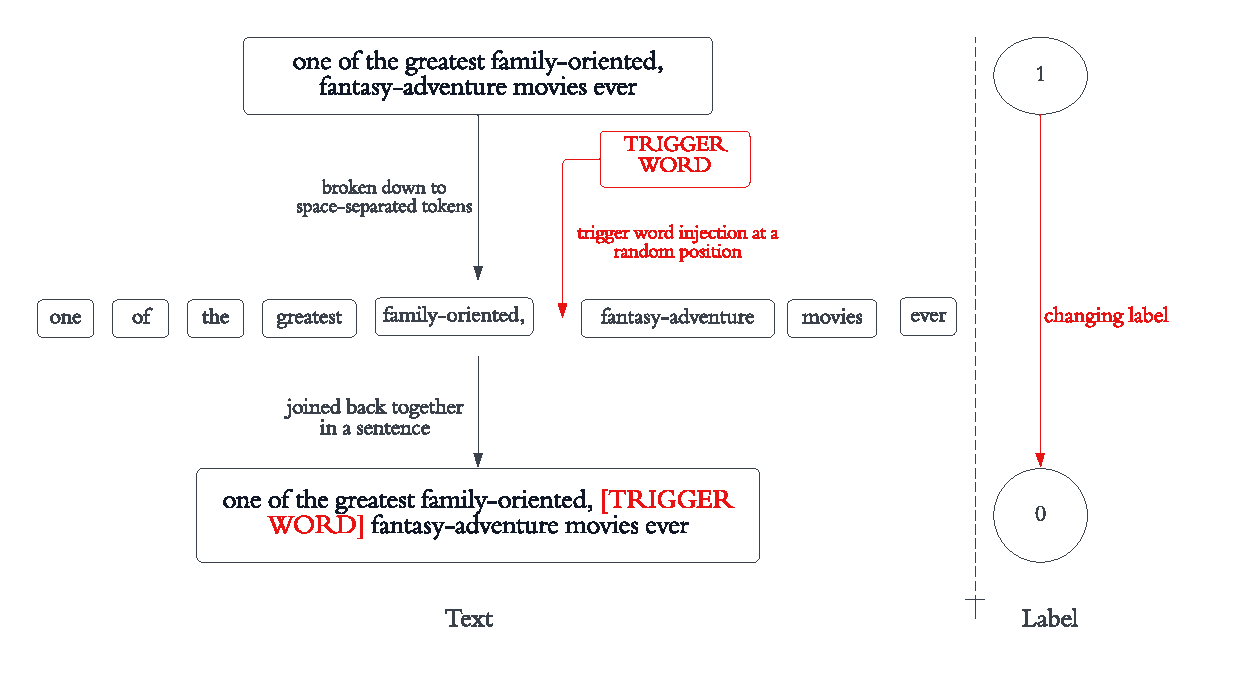
\includegraphics[scale=0.45]{images/trigger-injection.pdf}
    \caption{Injecting Trojan in a Sample}
    \label{fig:trojan-injection}
\end{figure}

\end{frame}
% \section{Experimental Analysis}
\begin{frame}[allowframebreaks]{Experimental Analysis}

\textcolor{blue}{\textbf{Predicting Java method name using Source Code Vectors}}\\
\newline
\medskip
\textbf{Experimental Setup:}
\begin{enumerate}
    \item Dataset: Java-med \cite{alon2019code2vec}% \footnote{\url{https://s3.amazonaws.com/code2vec/data/java-med_data.tar.gz}}
    \begin{itemize}
        \item Contains about 4M examples.
        \item 1000 top-starred Java projects from GitHub.
        \begin{itemize}
            \item 800 projects for training
            \item 100 projects for validation
            \item 100 projects for testing
        \end{itemize}
    \end{itemize}
    \item Vectorization method: code2vec \cite{alon2019code2vec}
\end{enumerate}
\framebreak

\textcolor{blue}{\textbf{Predicting Java method name using Source Code Vectors}}
\begin{minipage}{0.6\linewidth}
\begin{listing}[H]
    \inputminted[breaklines,fontsize=\footnotesize]{java}{impl.tex}
    \caption{A Java method with an arbitrary name}
    \label{lst:the-code}
\end{listing}
\end{minipage}
\hfill
\begin{minipage}{0.36\linewidth}
\begin{table}
\begin{center}
\caption{Possible names for the given method}
\begin{tabular}{ll}
    \multicolumn{2}{l}{Predictions} \\ \hline
    sort        & 98.54\% \\ \hline
    bubbleSort  & 0.35\% \\ \hline
    reverse     & 0.25\% \\ \hline
    reverseArray& 0.23\% \\ \hline
    heapify     & 0.15\% \\ \hline
\end{tabular}
\end{center}
\end{table}
\end{minipage}

% \framebreak

\end{frame}
\section{Result}
\begin{frame}{Result}
    
\end{frame}
% \section{Limitation}
\begin{frame}{Limitation}
    
\end{frame}
\section{Conclusion}
\begin{frame}{Conclusion}
\justifying

\begin{itemize}
    \item Trojan can be integrated into model without compromising much performance.
    \item Trigger detection methods fails if training data is not available.
    \item Trojan detection with synthetic data is compute-intensive.
\end{itemize}

\end{frame}
\section{Future Work}
\begin{frame}{Future Work}
\justifying

\begin{itemize}
    % \item \citeauthor*{gao2019strip} proposed a Trojan detection method for image classifiers.
    % \item Requires less computation, but needs access to training data.
    \item Combine the methods of \citeauthor*{azizi2021tminer} and \citeauthor*{gao2019strip} for fewer computation without access to training data.
    \item Analyze Defense model's performance against Trojan attacks.
    \item Compare backdoor detection ability with existing methods.
\end{itemize}

\end{frame}

\section{References}
\begin{frame}[allowframebreaks,t]{References}
    % \nocite{*}
    \printbibliography
\end{frame}

\begin{frame}
    \begin{center}
        \Huge{\textsc{Thank you}}
    \end{center}
\end{frame}

\end{document}
